\documentclass{article}[18pt]
\usepackage{../../../../format}
\lhead{Networks and Systems - Networks}

% Right hand textbook on the slides is better to read
\begin{document}
\begin{center}
\underline{\huge Introduction}
\end{center}
\textbf{Computer Network} - A group of devices that are connected to one another in order to exchange information or share resources
\section{Overview}
\begin{center}
	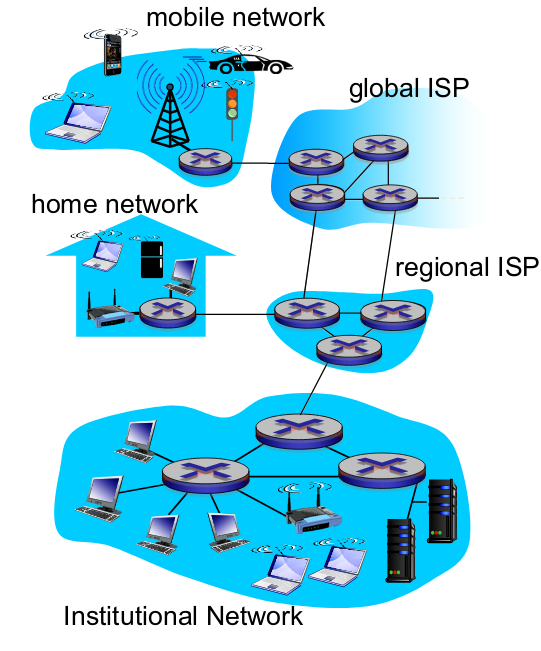
\includegraphics[scale=0.7]{Overview}
\end{center}
\textbf{Hosts} - End systems\\
\textbf{Communication links} - Fiber, copper, radio, satellite\\
\textbf{Bandwidth} - Transmission rate\\
\textbf{Packet switches} - Forward packets (routers and switches)\\
\textbf{Internet} - A network of networks\\
\textbf{Protocols} - Control sending, receiving of messages\\
\textbf{Internet standards}:
\begin{itemize}
	\item RFC: Request for comments
	\item IETF: Internet Engineering Task Force
\end{itemize}
\section{What's a protocol}
Protocols define the format and order of messages sent and received among network entities, and actions taken on message transmission and receipt
\section{Access Network}
\subsection{DSL}
Use existing telephone line to central office DSLAM
\begin{itemize}
	\item data over DSL phone line goes to internet
	\item voice over DSL phone line goes to telephone net
\end{itemize}
Asymmetric so much faster download than upload
\subsection{Cable network}
\begin{center}
	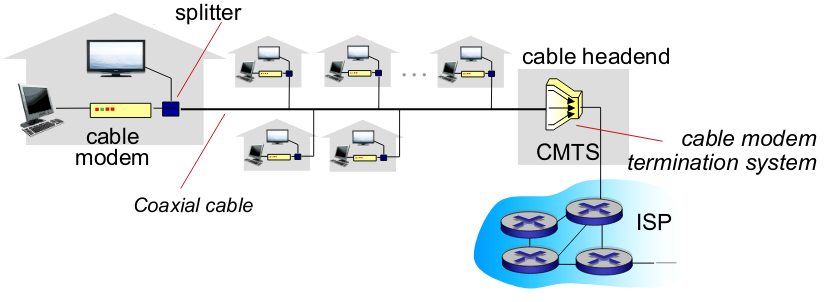
\includegraphics[scale=0.7]{Cable}
\end{center}
HFC - hybrid fiber coax\\
Network of cable, fiber attaches hones to ISP router
\begin{itemize}
	\item Homes share access network to cable headend
	\item Unlike DSL, which has dedicated access to central office
\end{itemize}
Shared line between a group of users\\
CMTS translates signal between the coaxial cable and the ISP
\subsection{Ethernet (Enterprise access networks)}
\begin{center}
	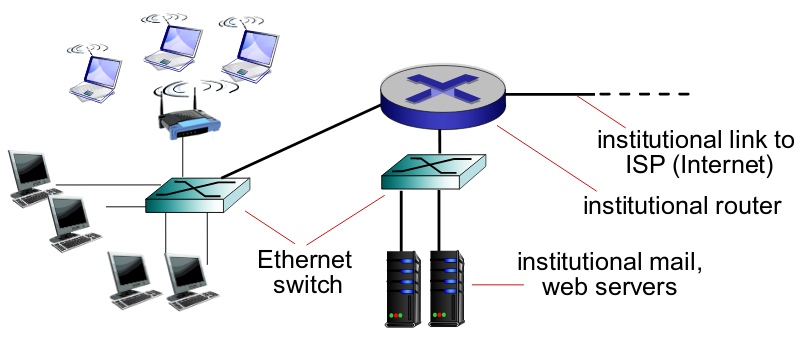
\includegraphics[scale=0.7]{Ethernet}
\end{center}
\subsection{Home network}
\begin{center}
	\includegraphics[scale=0.7]{"Home Network"}
\end{center}

\section{Wireless Access Networks}
Shared wireless access networks connects end system to router via base station, aka "access point"\\
\\
\textbf{Wireless LANs(802.11):} - Within Building (54-1300 Mbps)\\
\textbf{Wide-area wireless access} - 10s of km (1-10 Mbps)
\section{Physical media}
\textbf{Bit}:  Propagates between transmitter/reciever pairs\\
\textbf{Physical link}: What lies between the transmitter and reciever\\
\textbf{Guided media}: Signals propagate in solid media (usually cables or fibers)\\
\textbf{Unguided media}: Signals propagate freely (radio etc)
\subsection{Coax, Fiber}
\textbf{Twisted Pair}:
\begin{itemize}
	\item Two insulated copper wires
	\item Cat5: 10Mbps, 1Gbps
	\item Cat6: 10Gbps
\end{itemize}
\textbf{Coaxial cable}:
\begin{itemize}
	\item Two concentric copper conductors
	\item Can achieve high data transmission rates
\end{itemize}
\textbf{Fiber optic cable}
\begin{itemize}
	\item Glass fibre carrying light pulses representing bits
	\item High speed operation
	\item Low error rate
\end{itemize}
\subsection{Radio}
\begin{itemize}
	\item Signal carried in electromagnetic spectrum
	\item No physical wire
	\item Carry a signal for long distances
	\item Propagation environment effects
	\begin{itemize}
		\item Reflection
		\item Obstruction by objects
		\item Interference
	\end{itemize}
\end{itemize}
Classified into three groups
\begin{itemize}
	\item Very short distance
	\item LAN
	\item Wide area
\end{itemize}
\section{Network Security}
\textbf{Network Security}
\begin{itemize}
	\item How bad actors can attack computer networks
	\item How to defend networks against attacks
	\item How to design architectures resistant to attacks
\end{itemize}
\textbf{Internet originally designed with little security}
\begin{itemize}
	\item Original vision: "a group of mutually trusting users attached to a transparent network"
	\item Internet protocol designers playing "catch up"
	\item Security considerations in all layers
\end{itemize}
\textbf{Bad actors can "sniff" packets}
\begin{itemize}
	\item Broadcast media
	\item "Promiscuous" network interface reads/records all packets
\end{itemize}



\end{document}